\subsection{Безопасность жизнедеятельности}
	
	\subsubsection{Аннотация}

		Курс <<Безопасность жизнедеятельности>> получил смешанные отзывы.

		Лекции Цыбикова В.Н. и специалиста по психологии получили крайне положительные отзывы у студентов. Совет студентов и аспирантов ФРКТ предлагает поощрить перечисленных преподавателей и увеличить количество лекций, проводимых ими.

		Также Совет студентов и аспирантов ФРКТ рекомендует чётко определить критерии оценивания и донести их до студентов в начале семестра.

	\subsubsection{Общий отзыв студентов о курсе}

		\begin{figure}[H]
			\centering
			\begin{subfigure}[b]{0.45\textwidth}
				\centering
				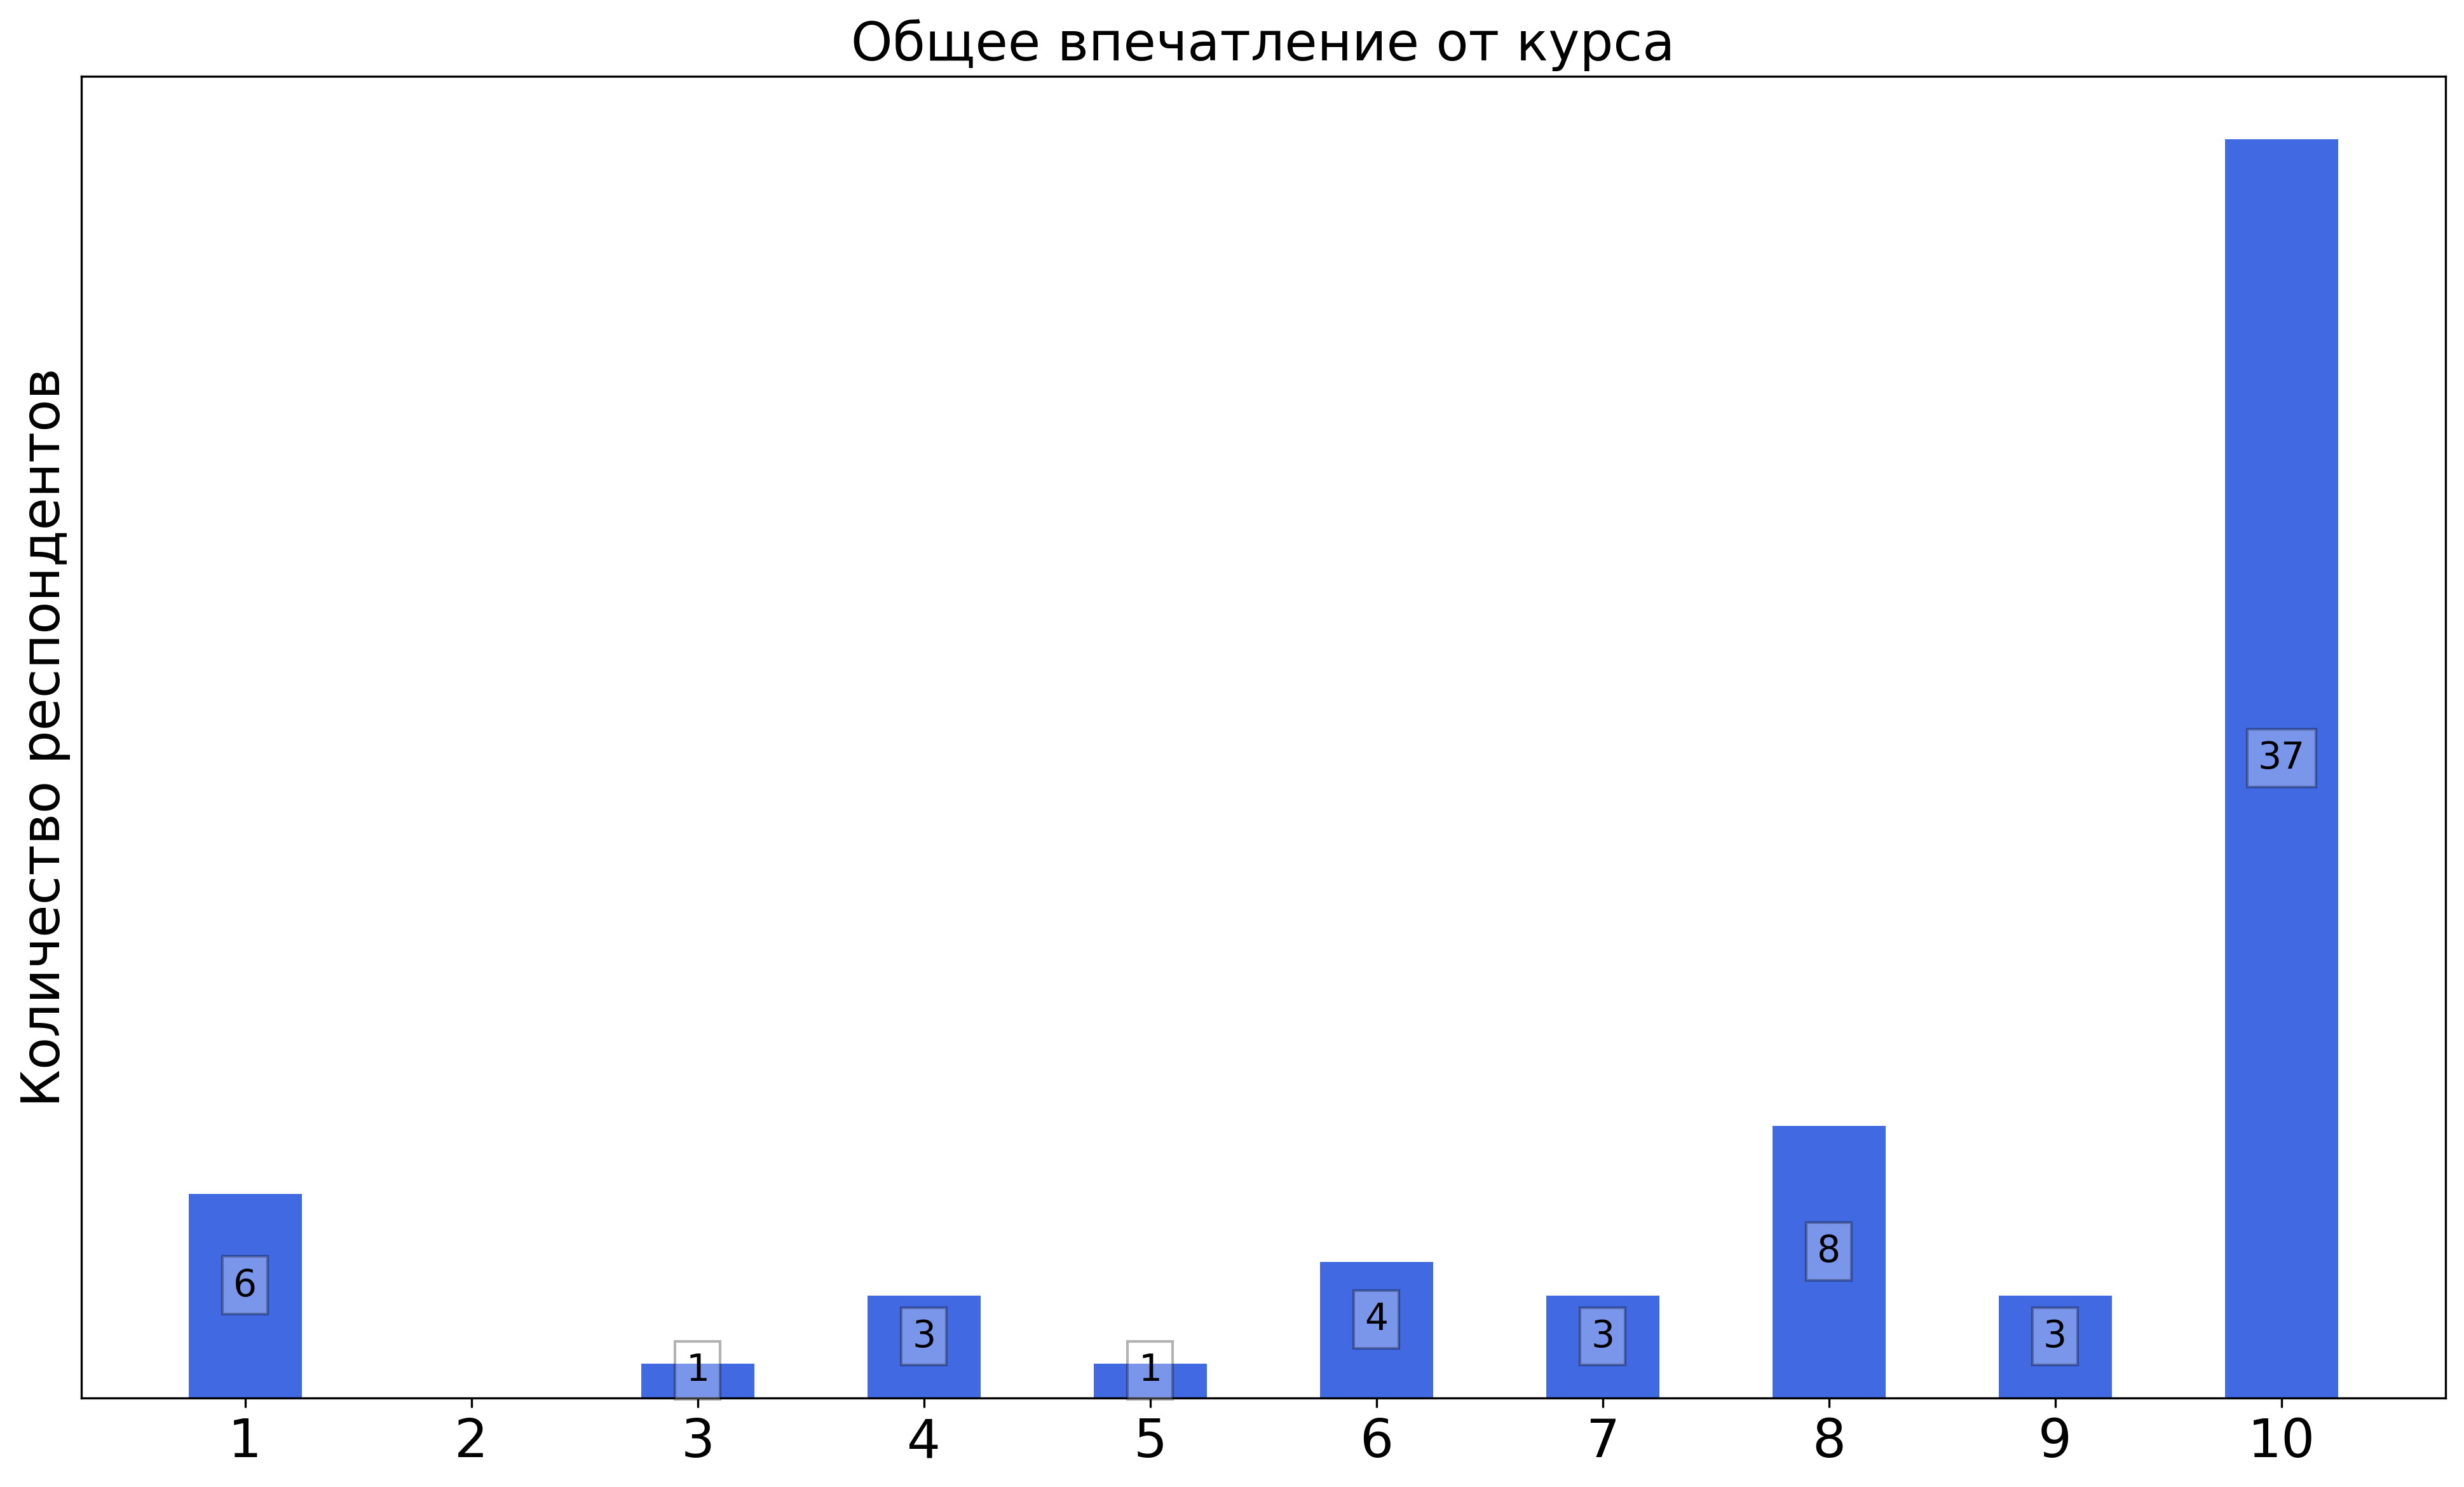
\includegraphics[width=\textwidth]{images/1 course/БЖД/general-0.png}
			\end{subfigure}
		\end{figure}

	\subsubsection{Материалы, использумые респондентами при изучении курса}

		\begin{figure}[H]
			\centering
			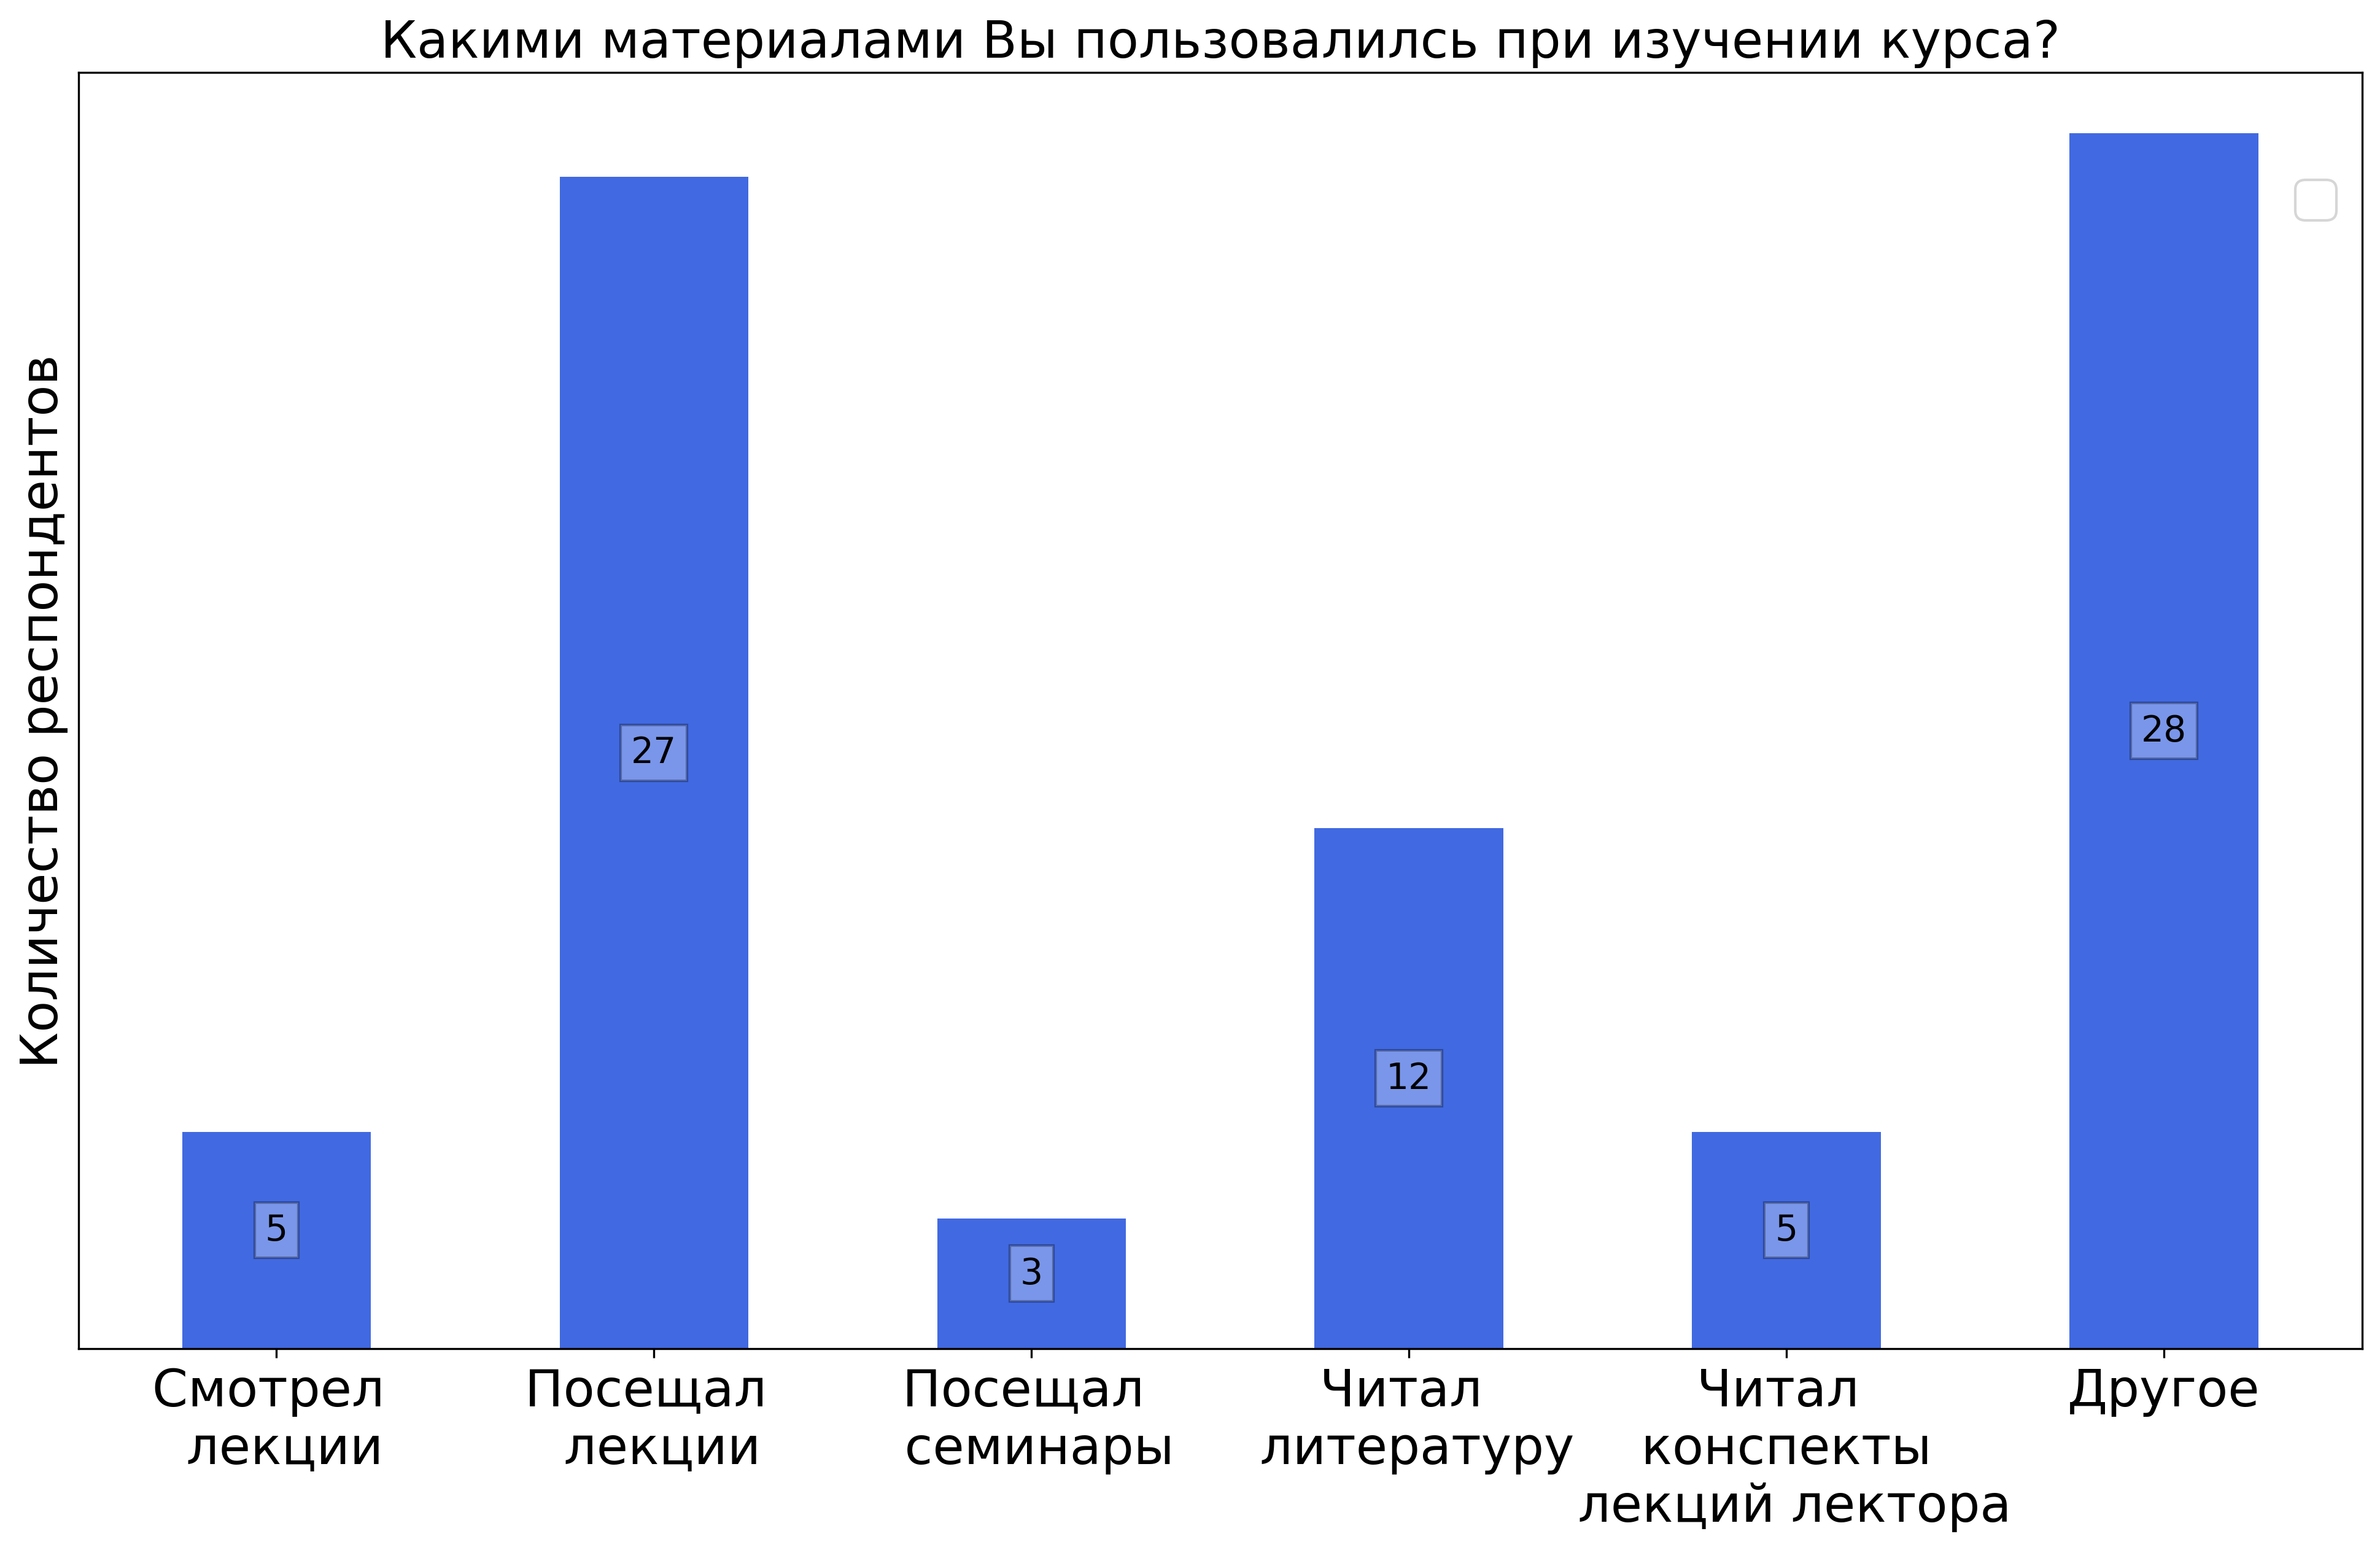
\includegraphics[width = 0.45\textwidth]{images/1 course/БЖД/materials.png}
		\end{figure}

		\textit{В качестве других источников информации студенты указали:} 
		\begin{itemize}
			\item материалы из интернета.
		\end{itemize}

	\subsubsection{Отзыв студентов о лекциях}

		\begin{figure}[H]
			\centering
            \begin{subfigure}[b]{0.45\textwidth}
				\centering
				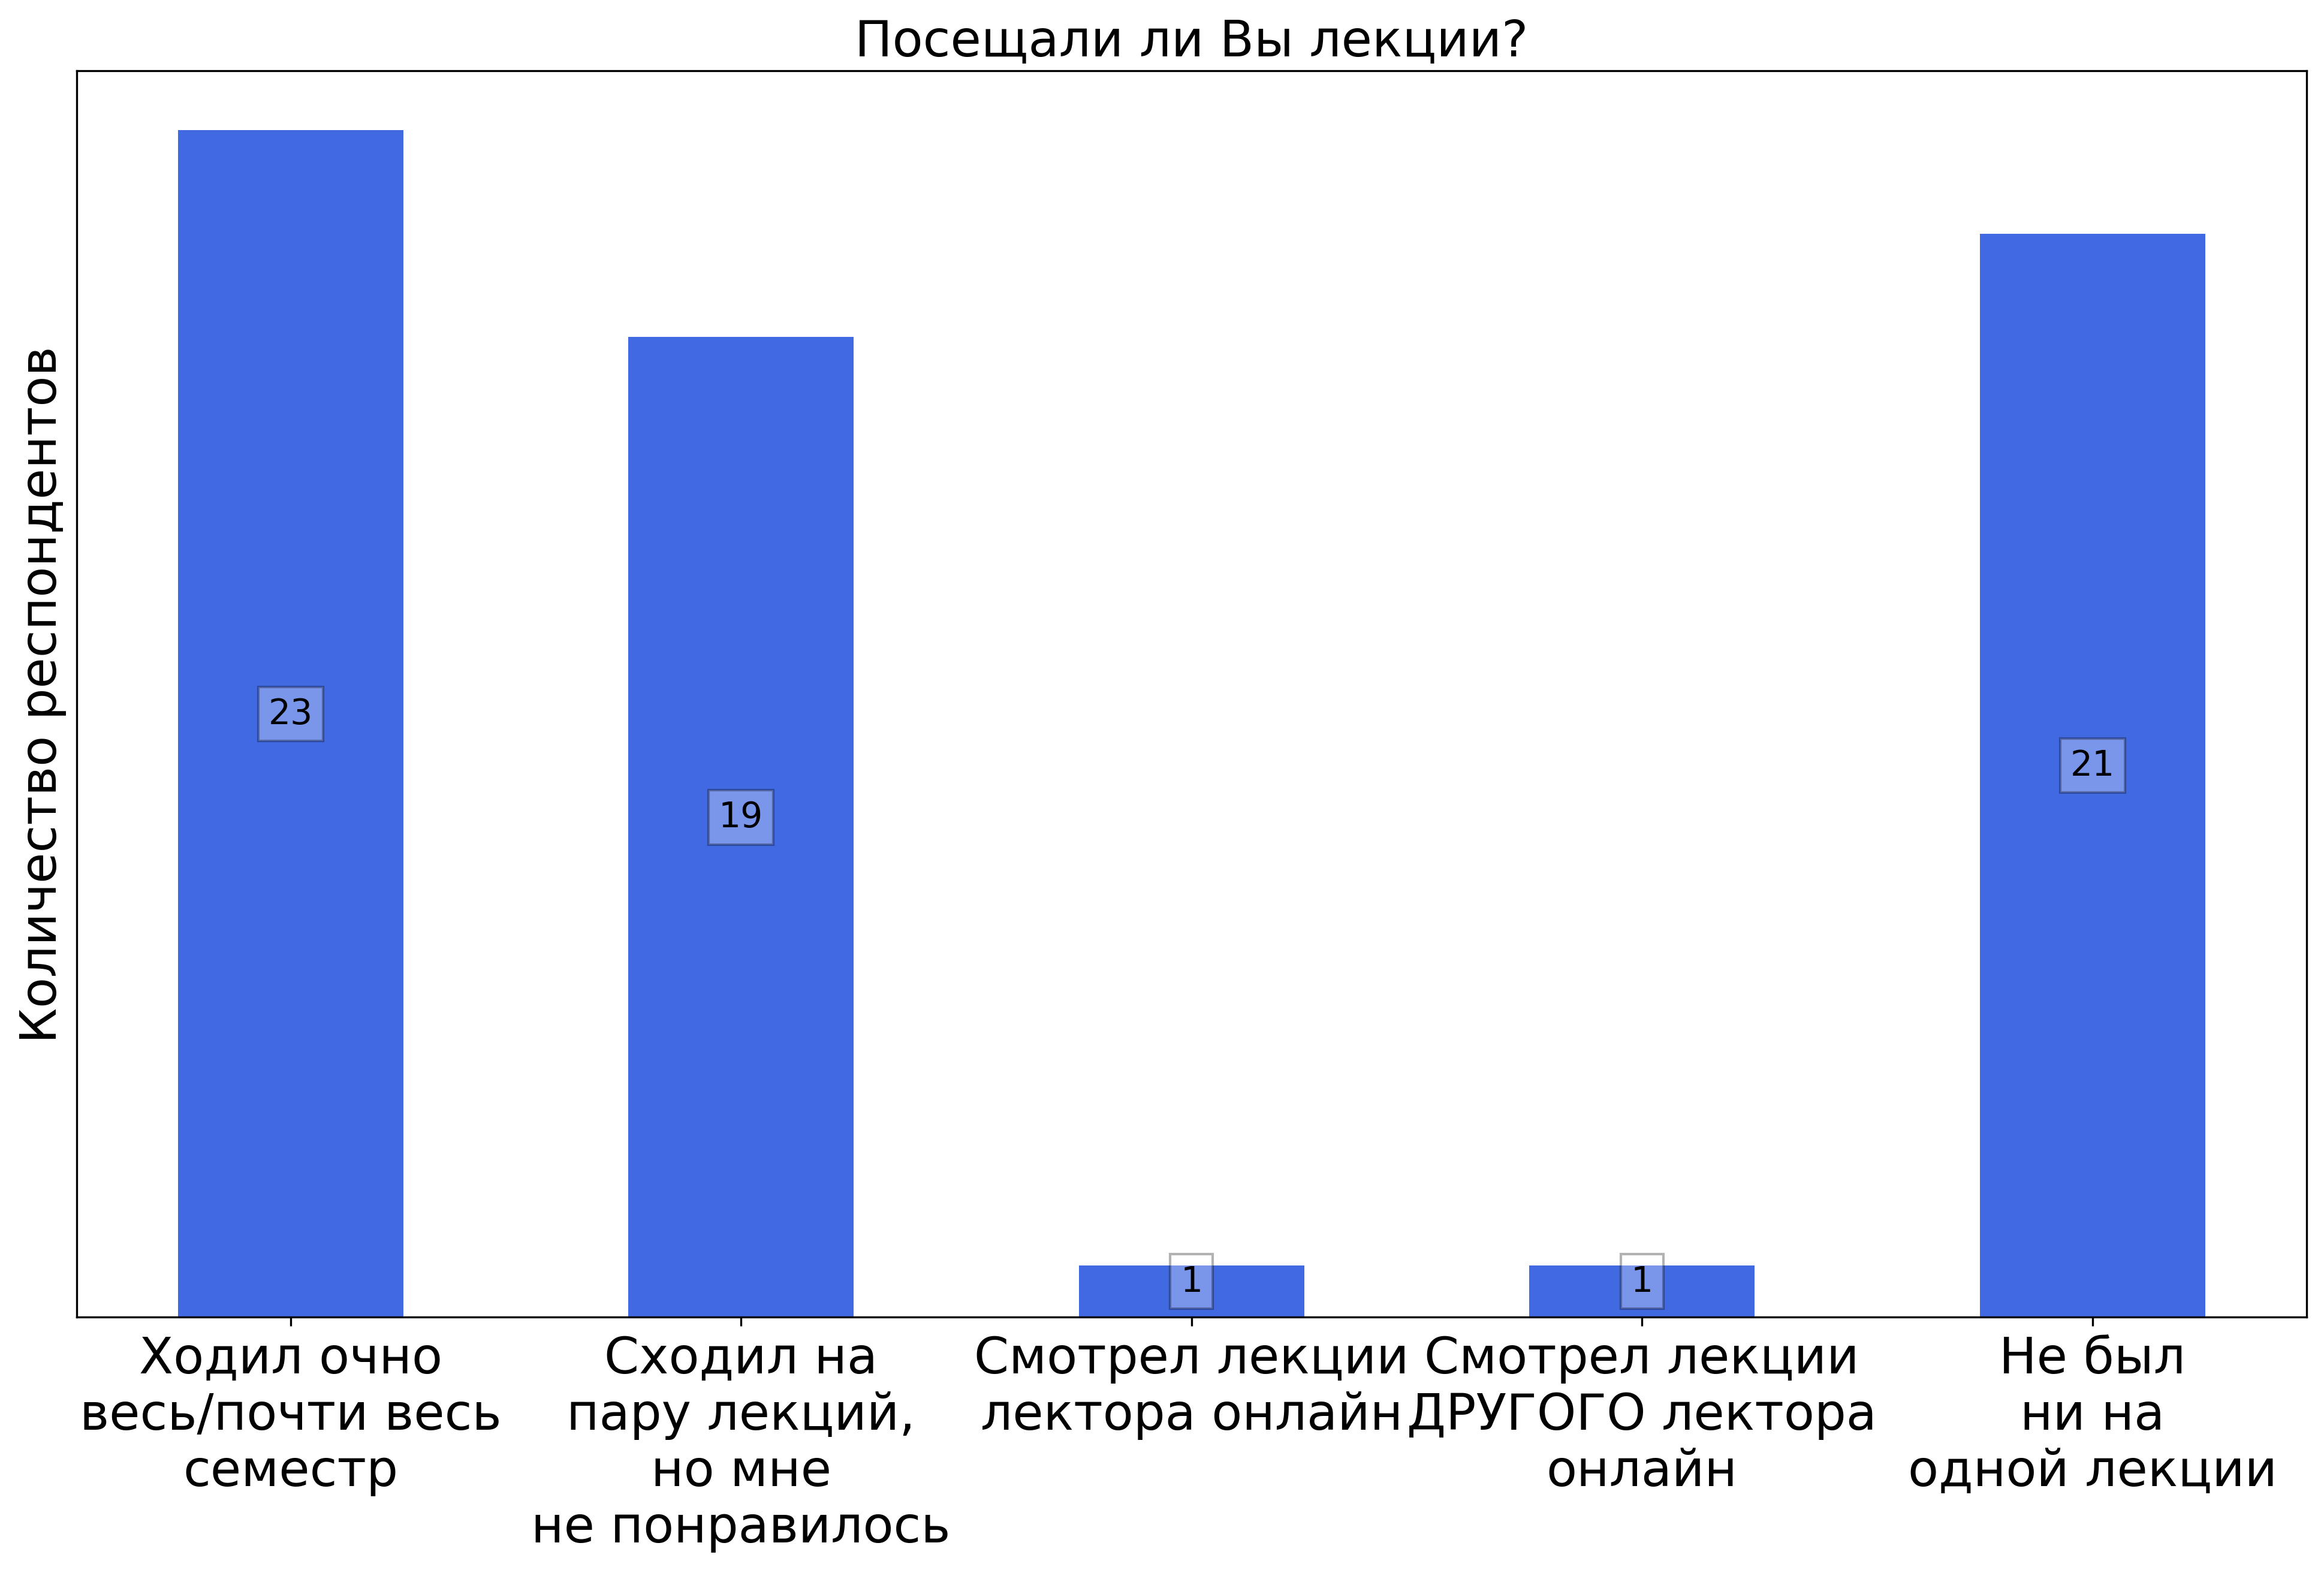
\includegraphics[width=\textwidth]{images/1 course/БЖД/lecturer-questions-0.png}
			\end{subfigure}
			\begin{subfigure}[b]{0.45\textwidth}
				\centering
				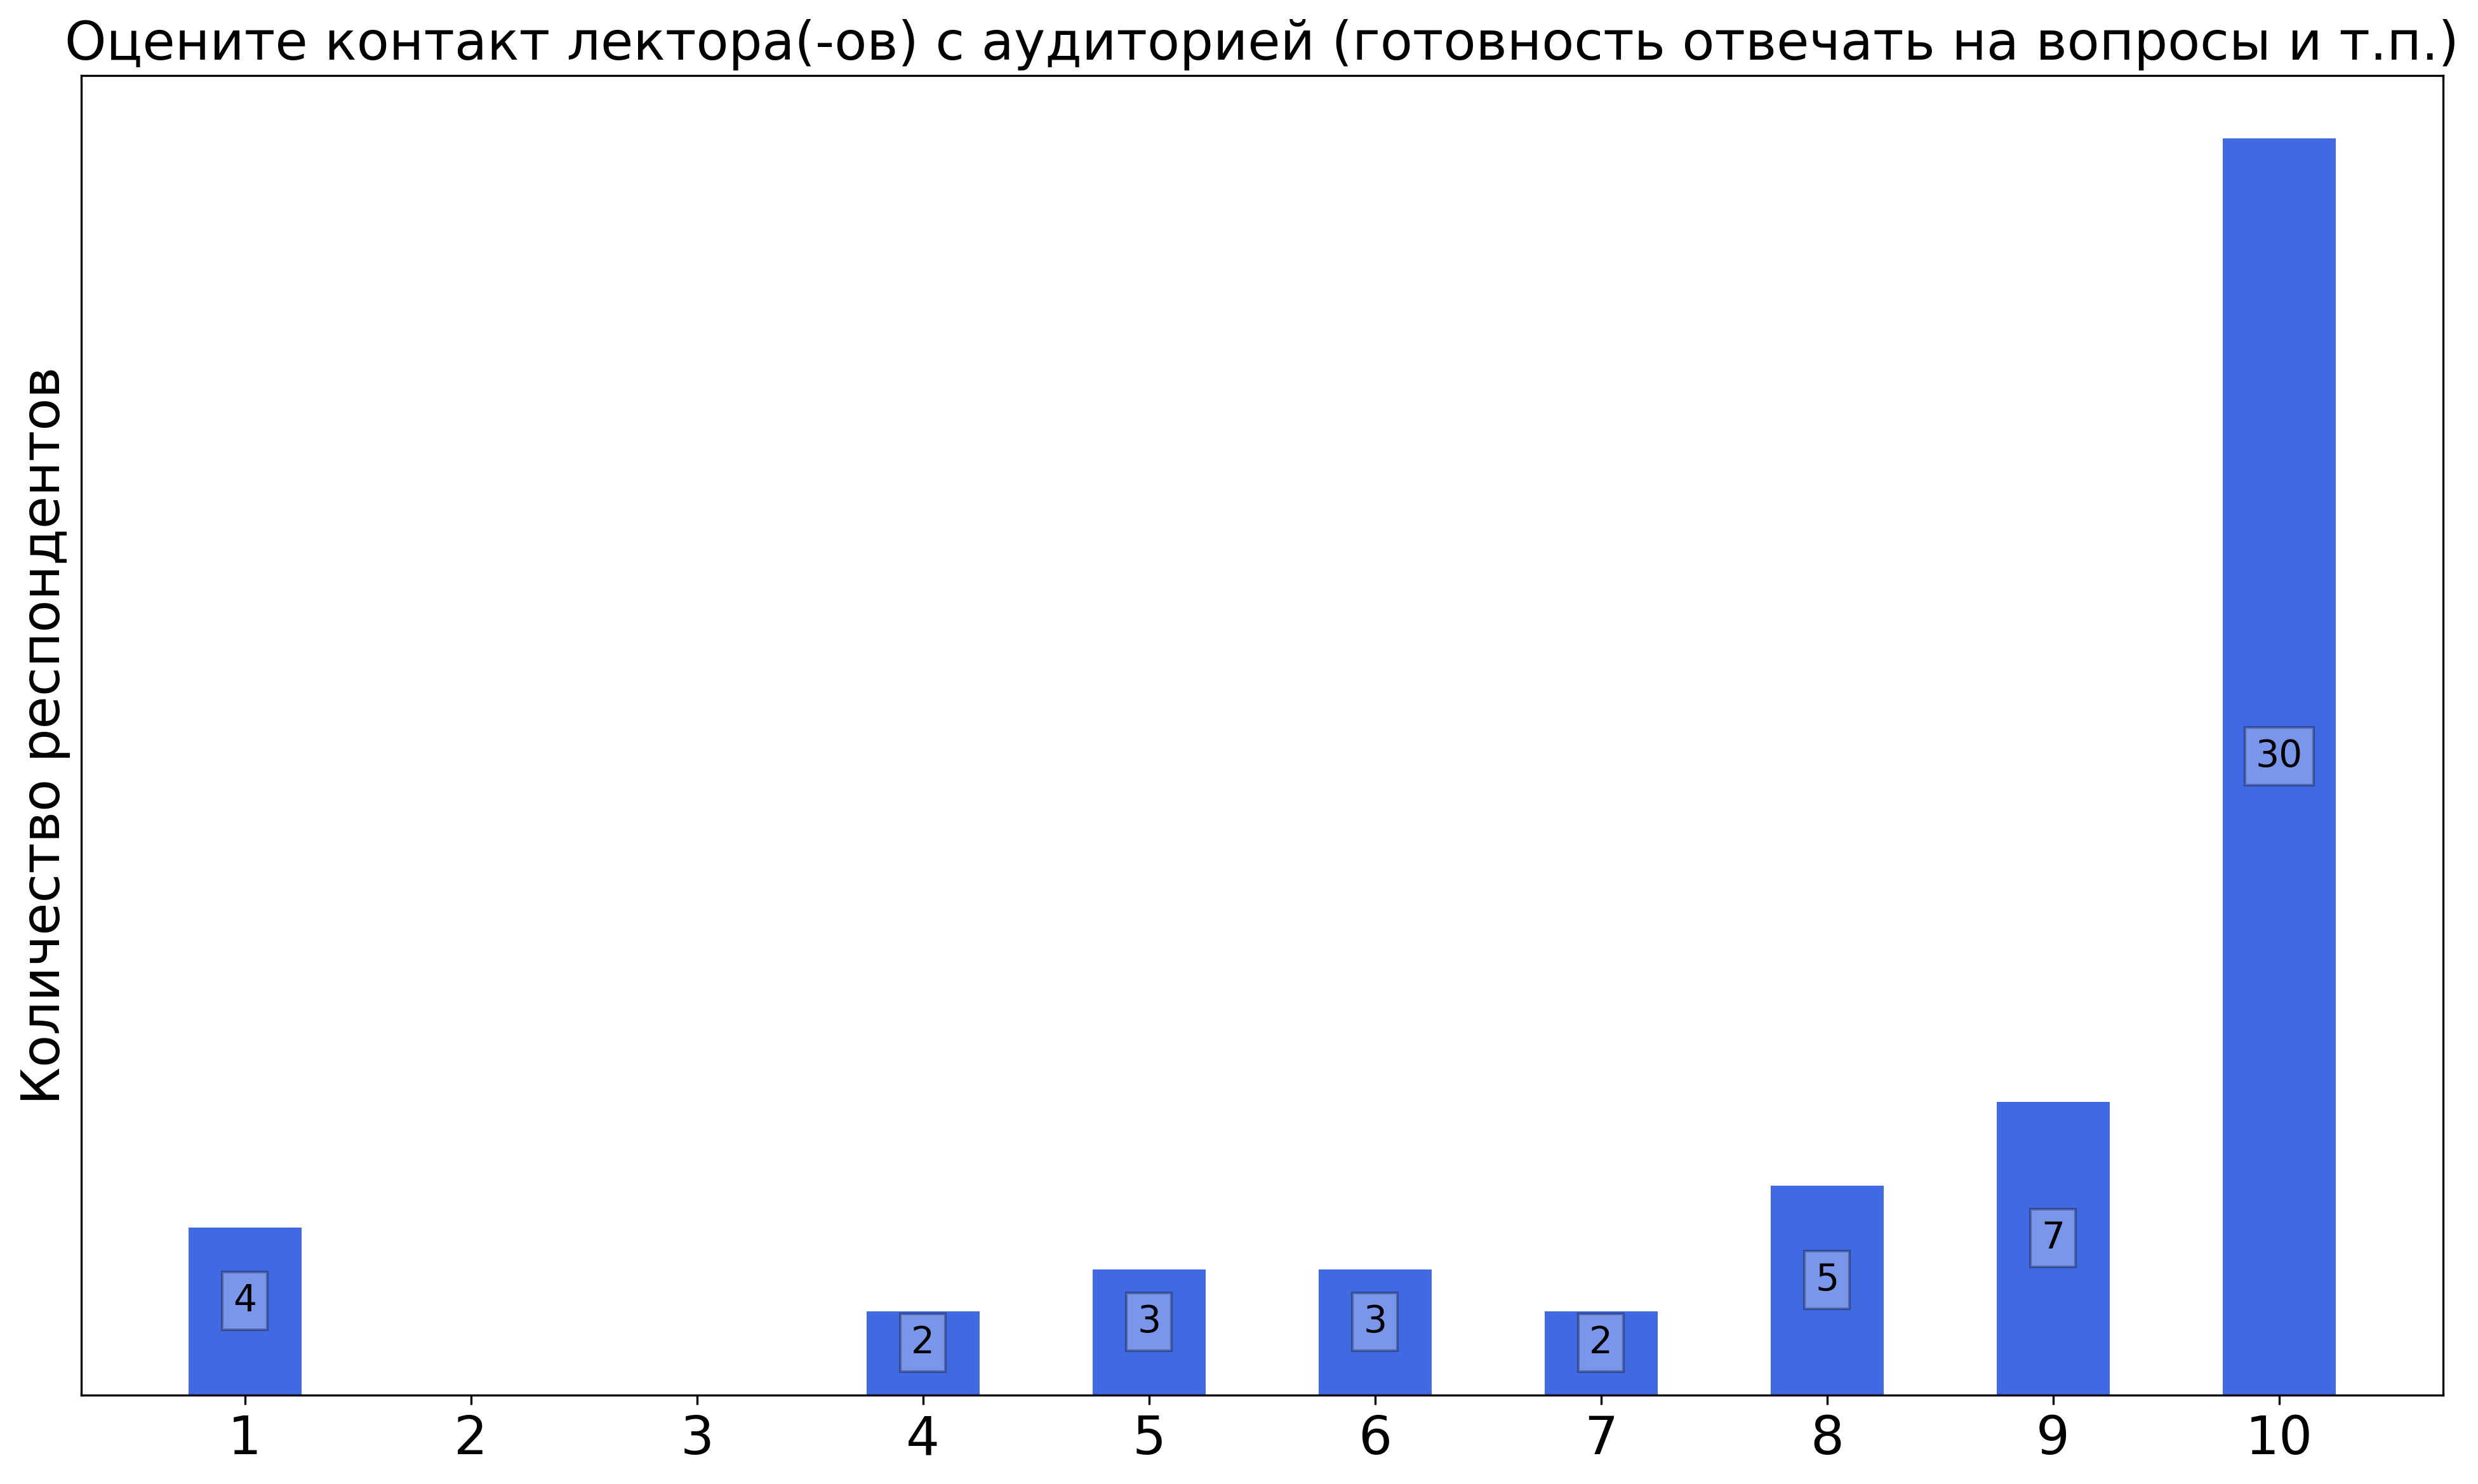
\includegraphics[width=\textwidth]{images/1 course/БЖД/lecturer-marks-0.png}
			\end{subfigure}
			\begin{subfigure}[b]{0.45\textwidth}
				\centering
				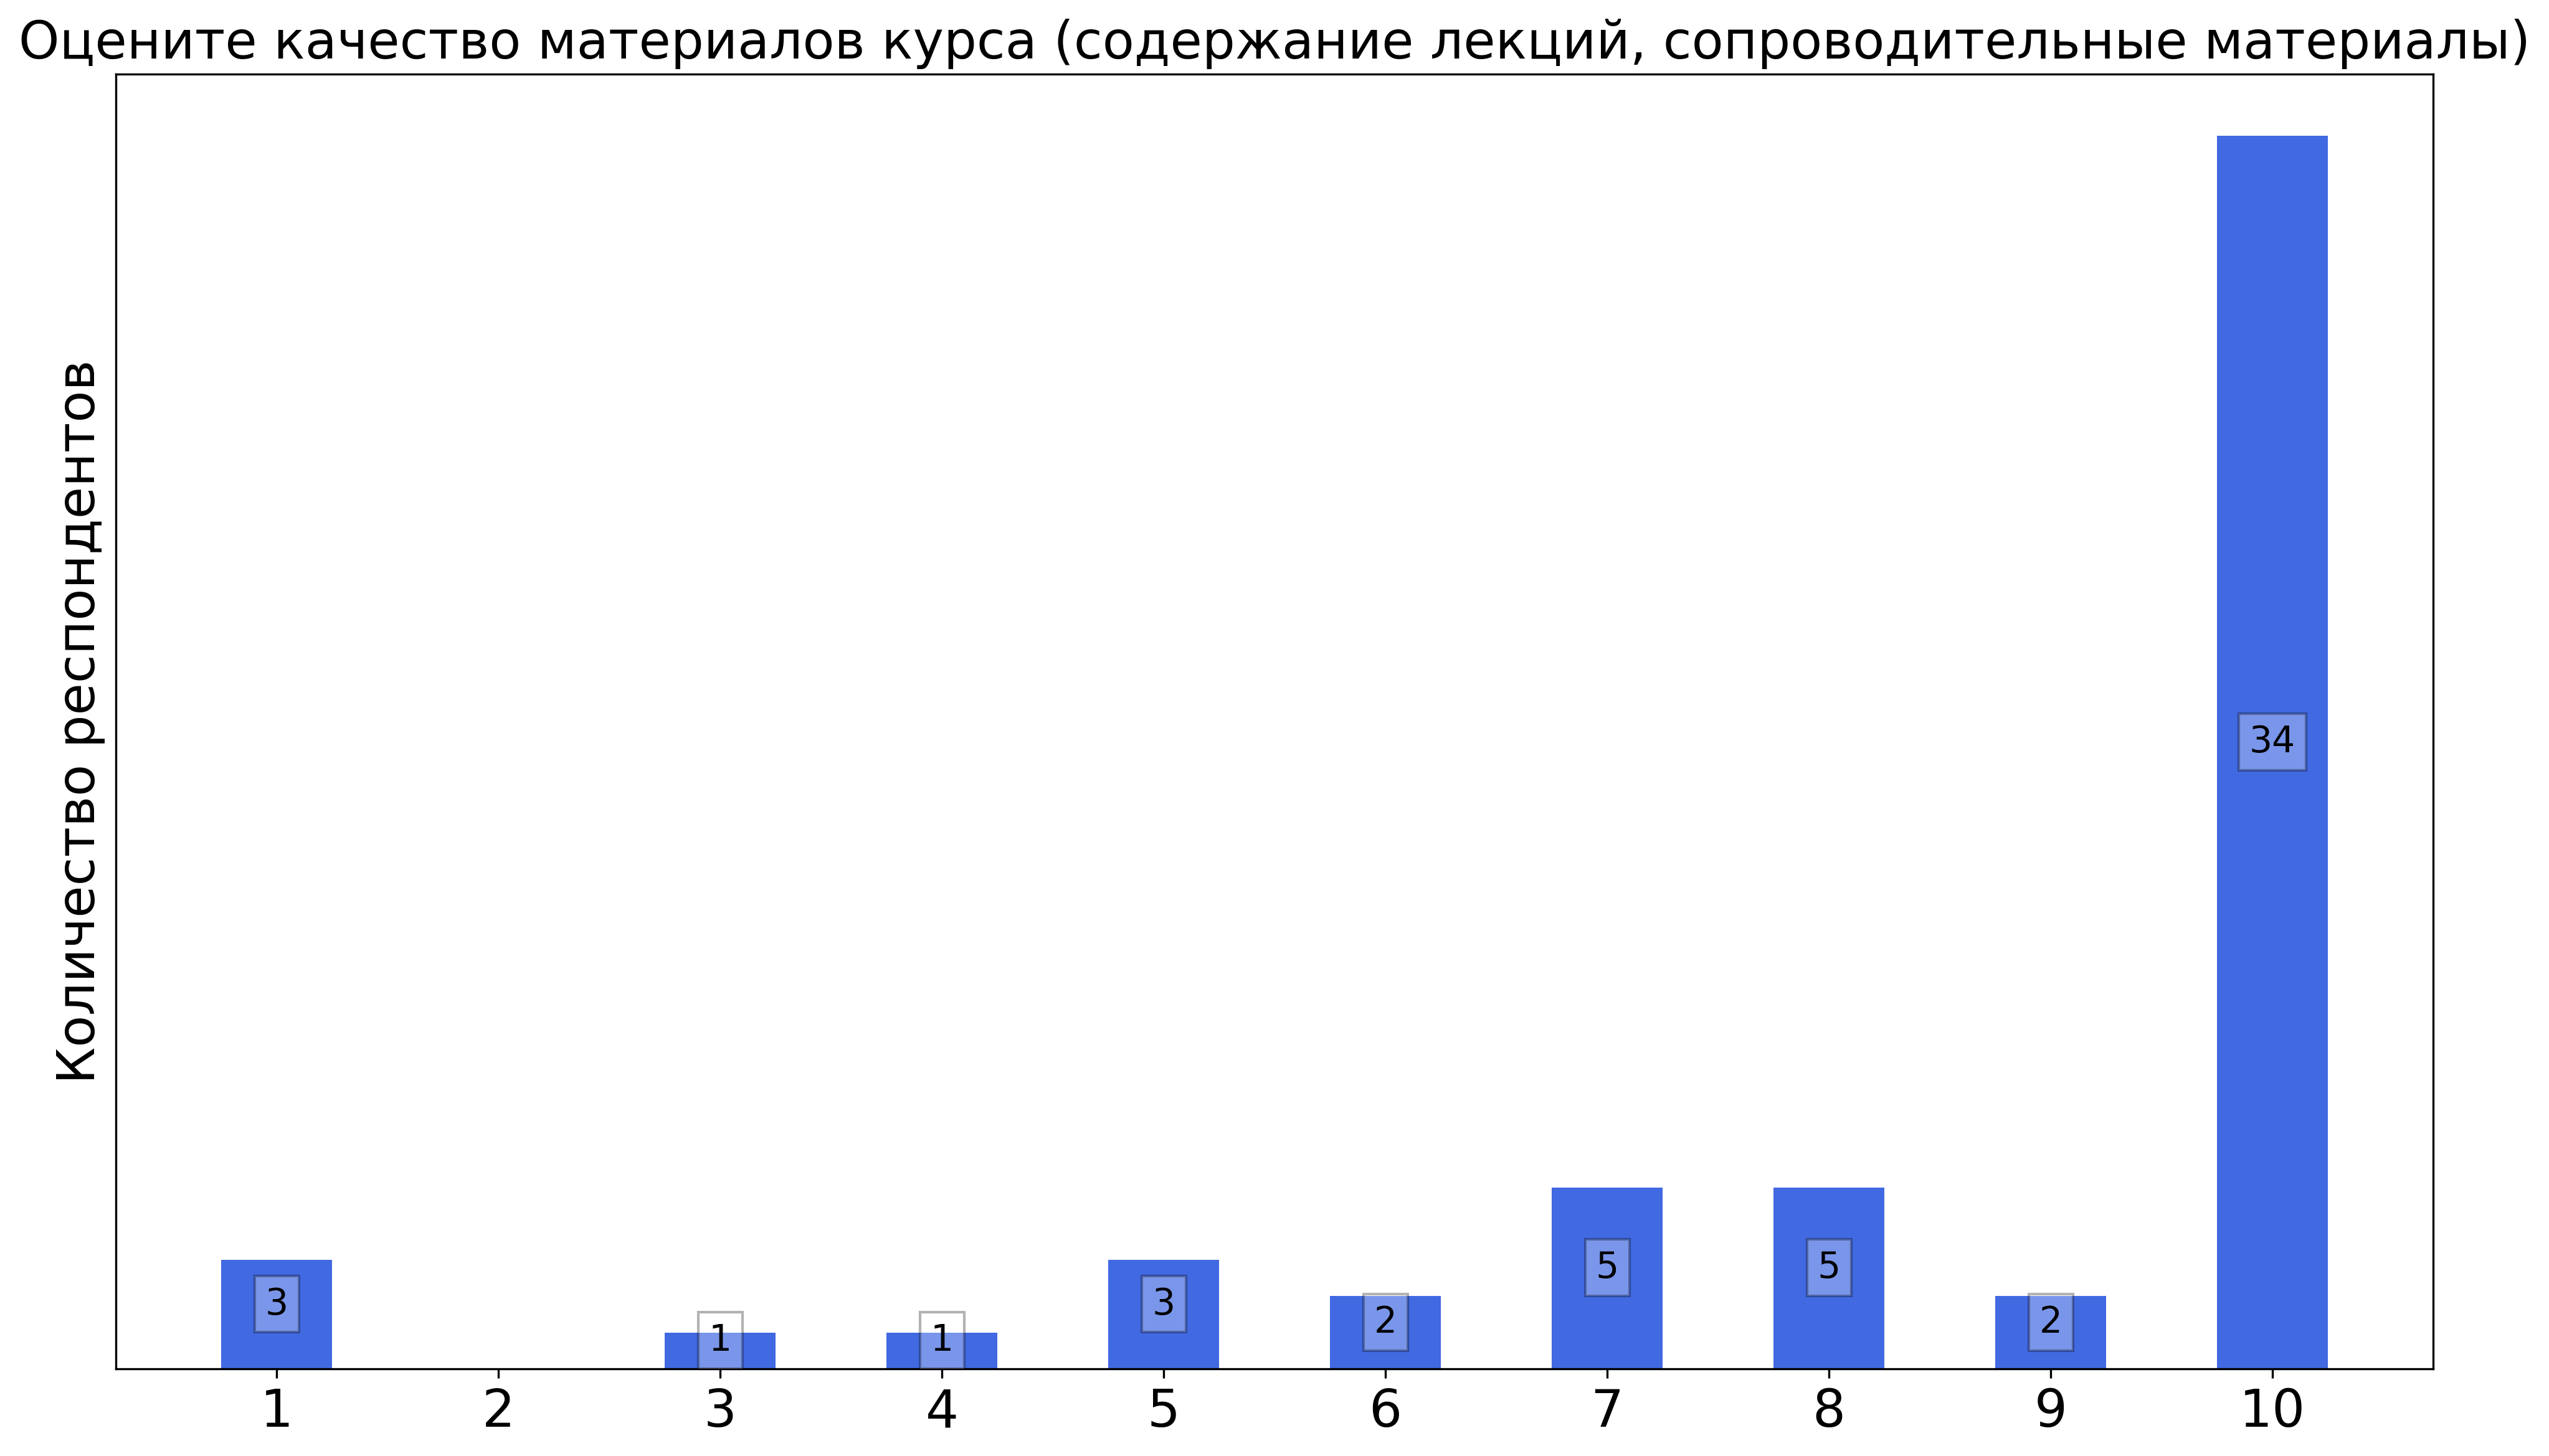
\includegraphics[width=\textwidth]{images/1 course/БЖД/lecturer-marks-1.png}
			\end{subfigure}
			\begin{subfigure}[b]{0.45\textwidth}
				\centering
				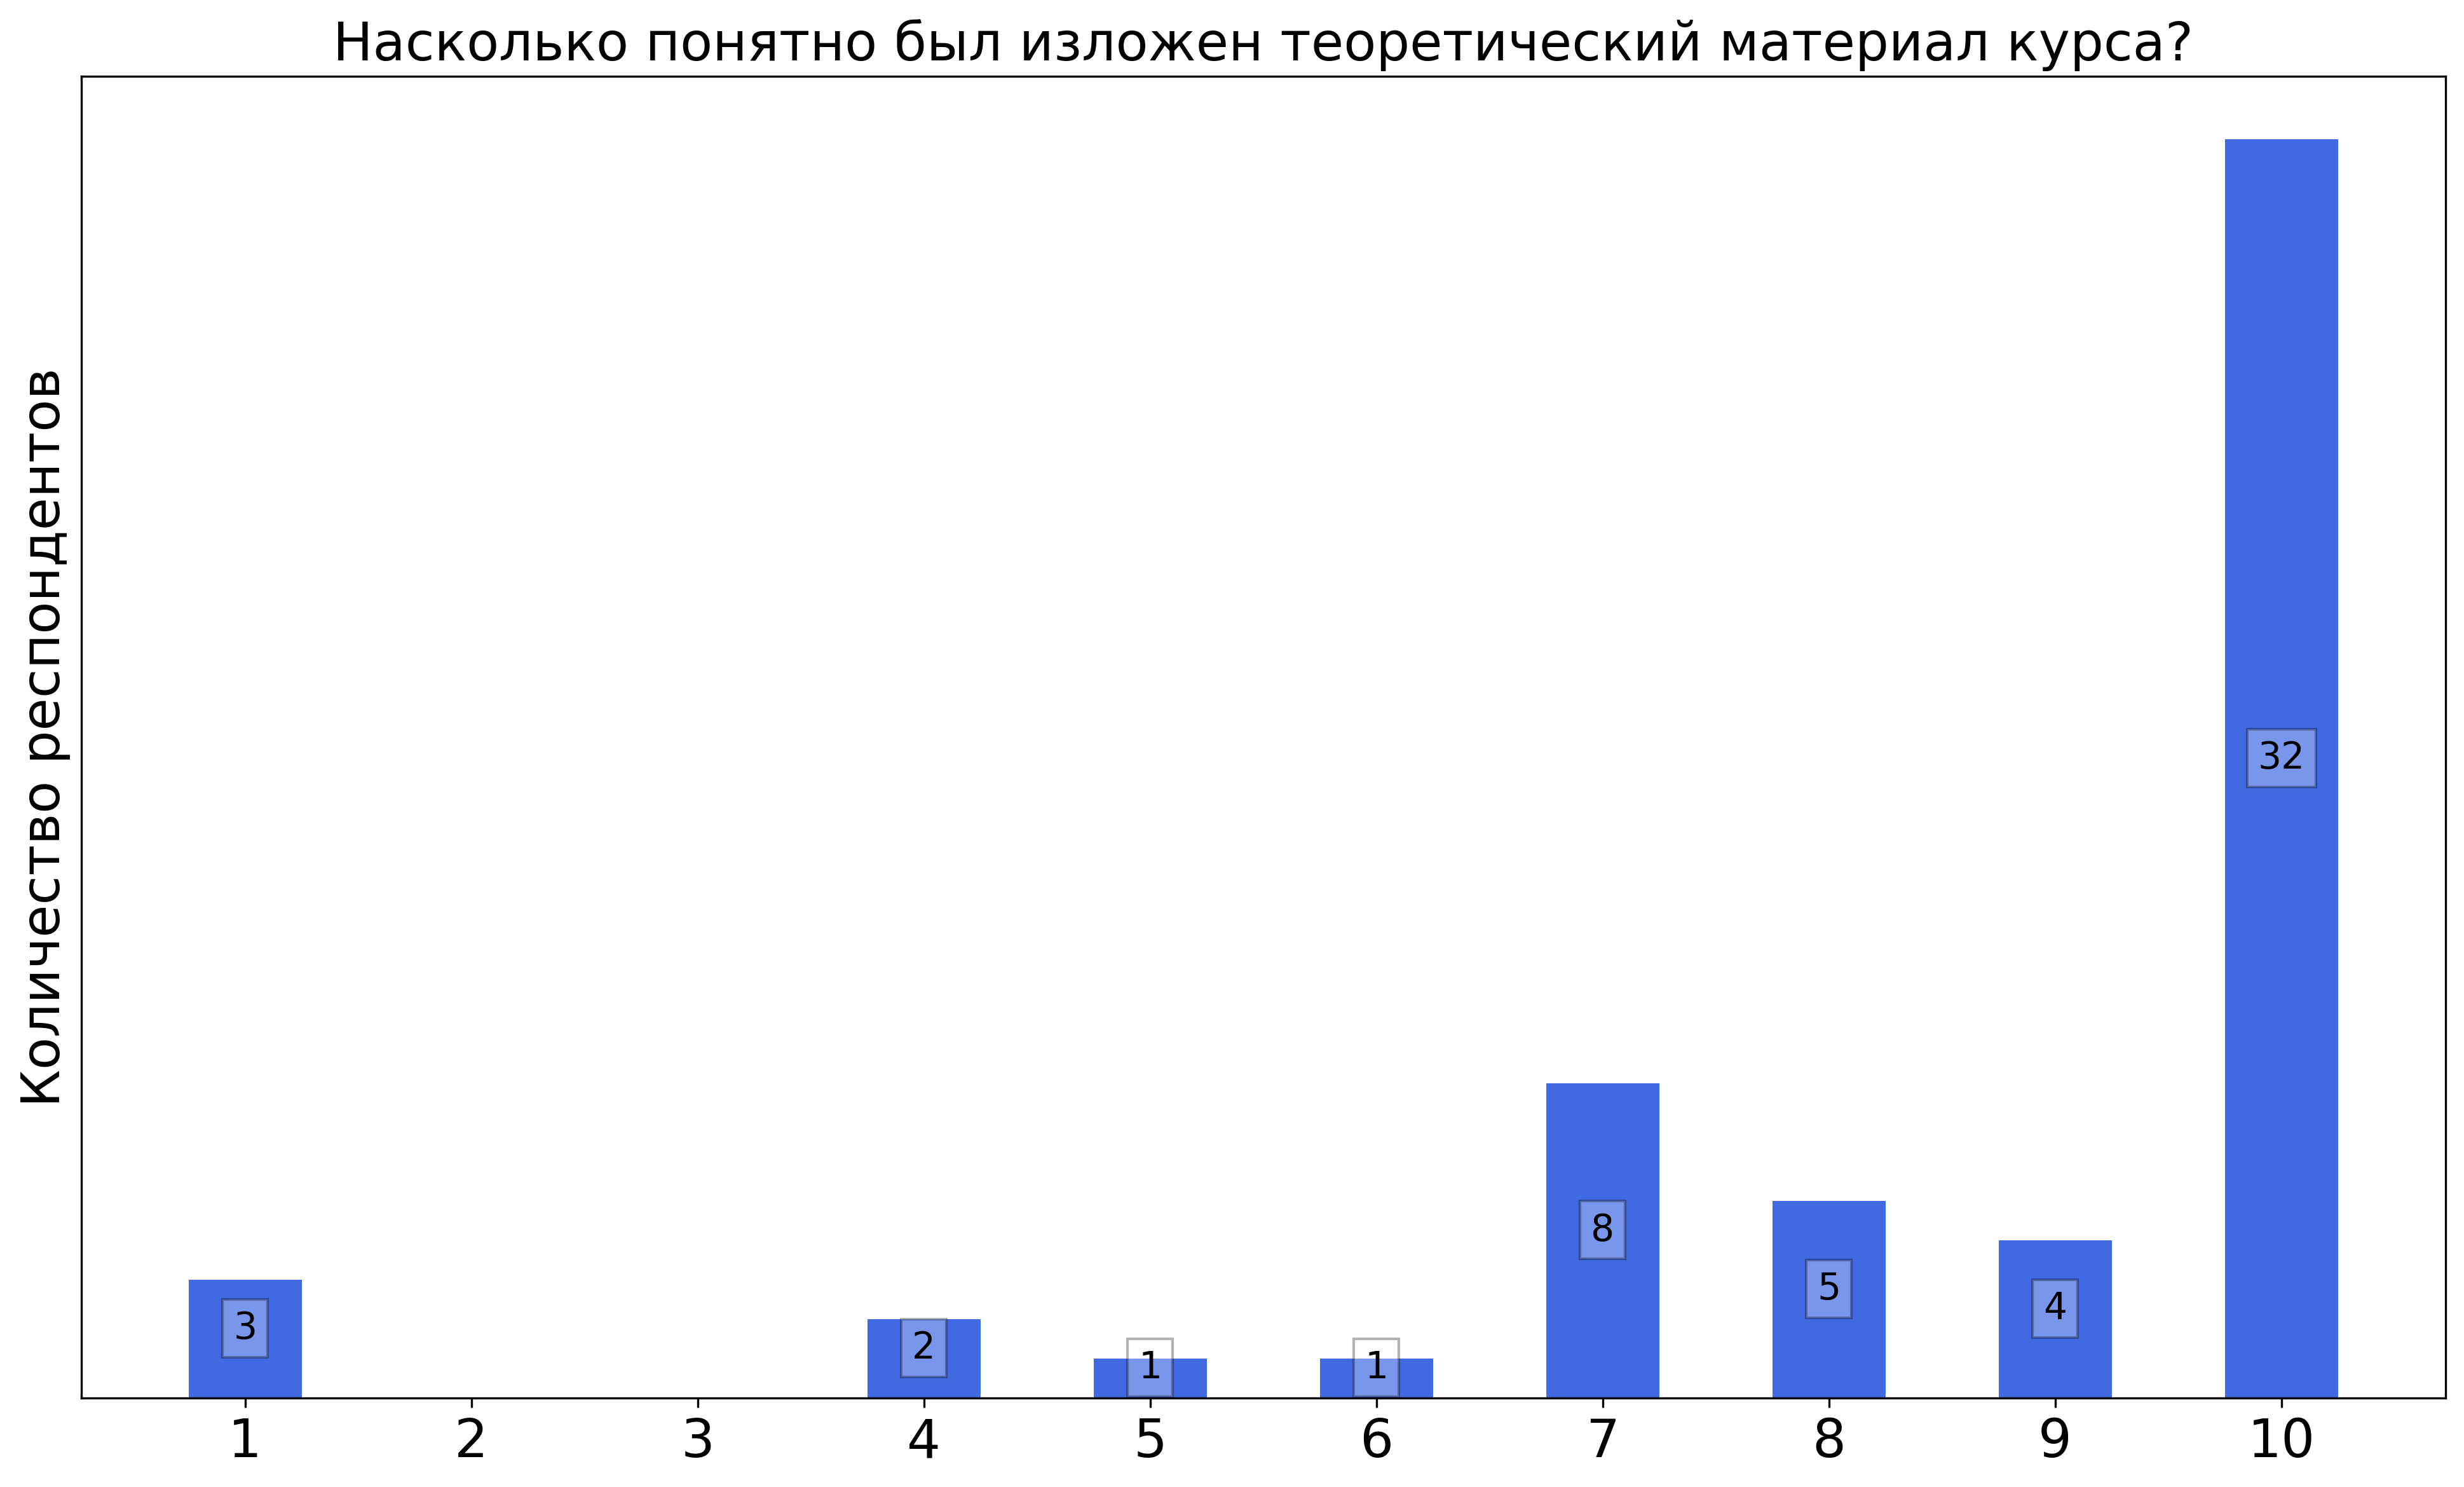
\includegraphics[width=\textwidth]{images/1 course/БЖД/lecturer-marks-2.png}
			\end{subfigure}	
			\begin{subfigure}[b]{0.45\textwidth}
				\centering
				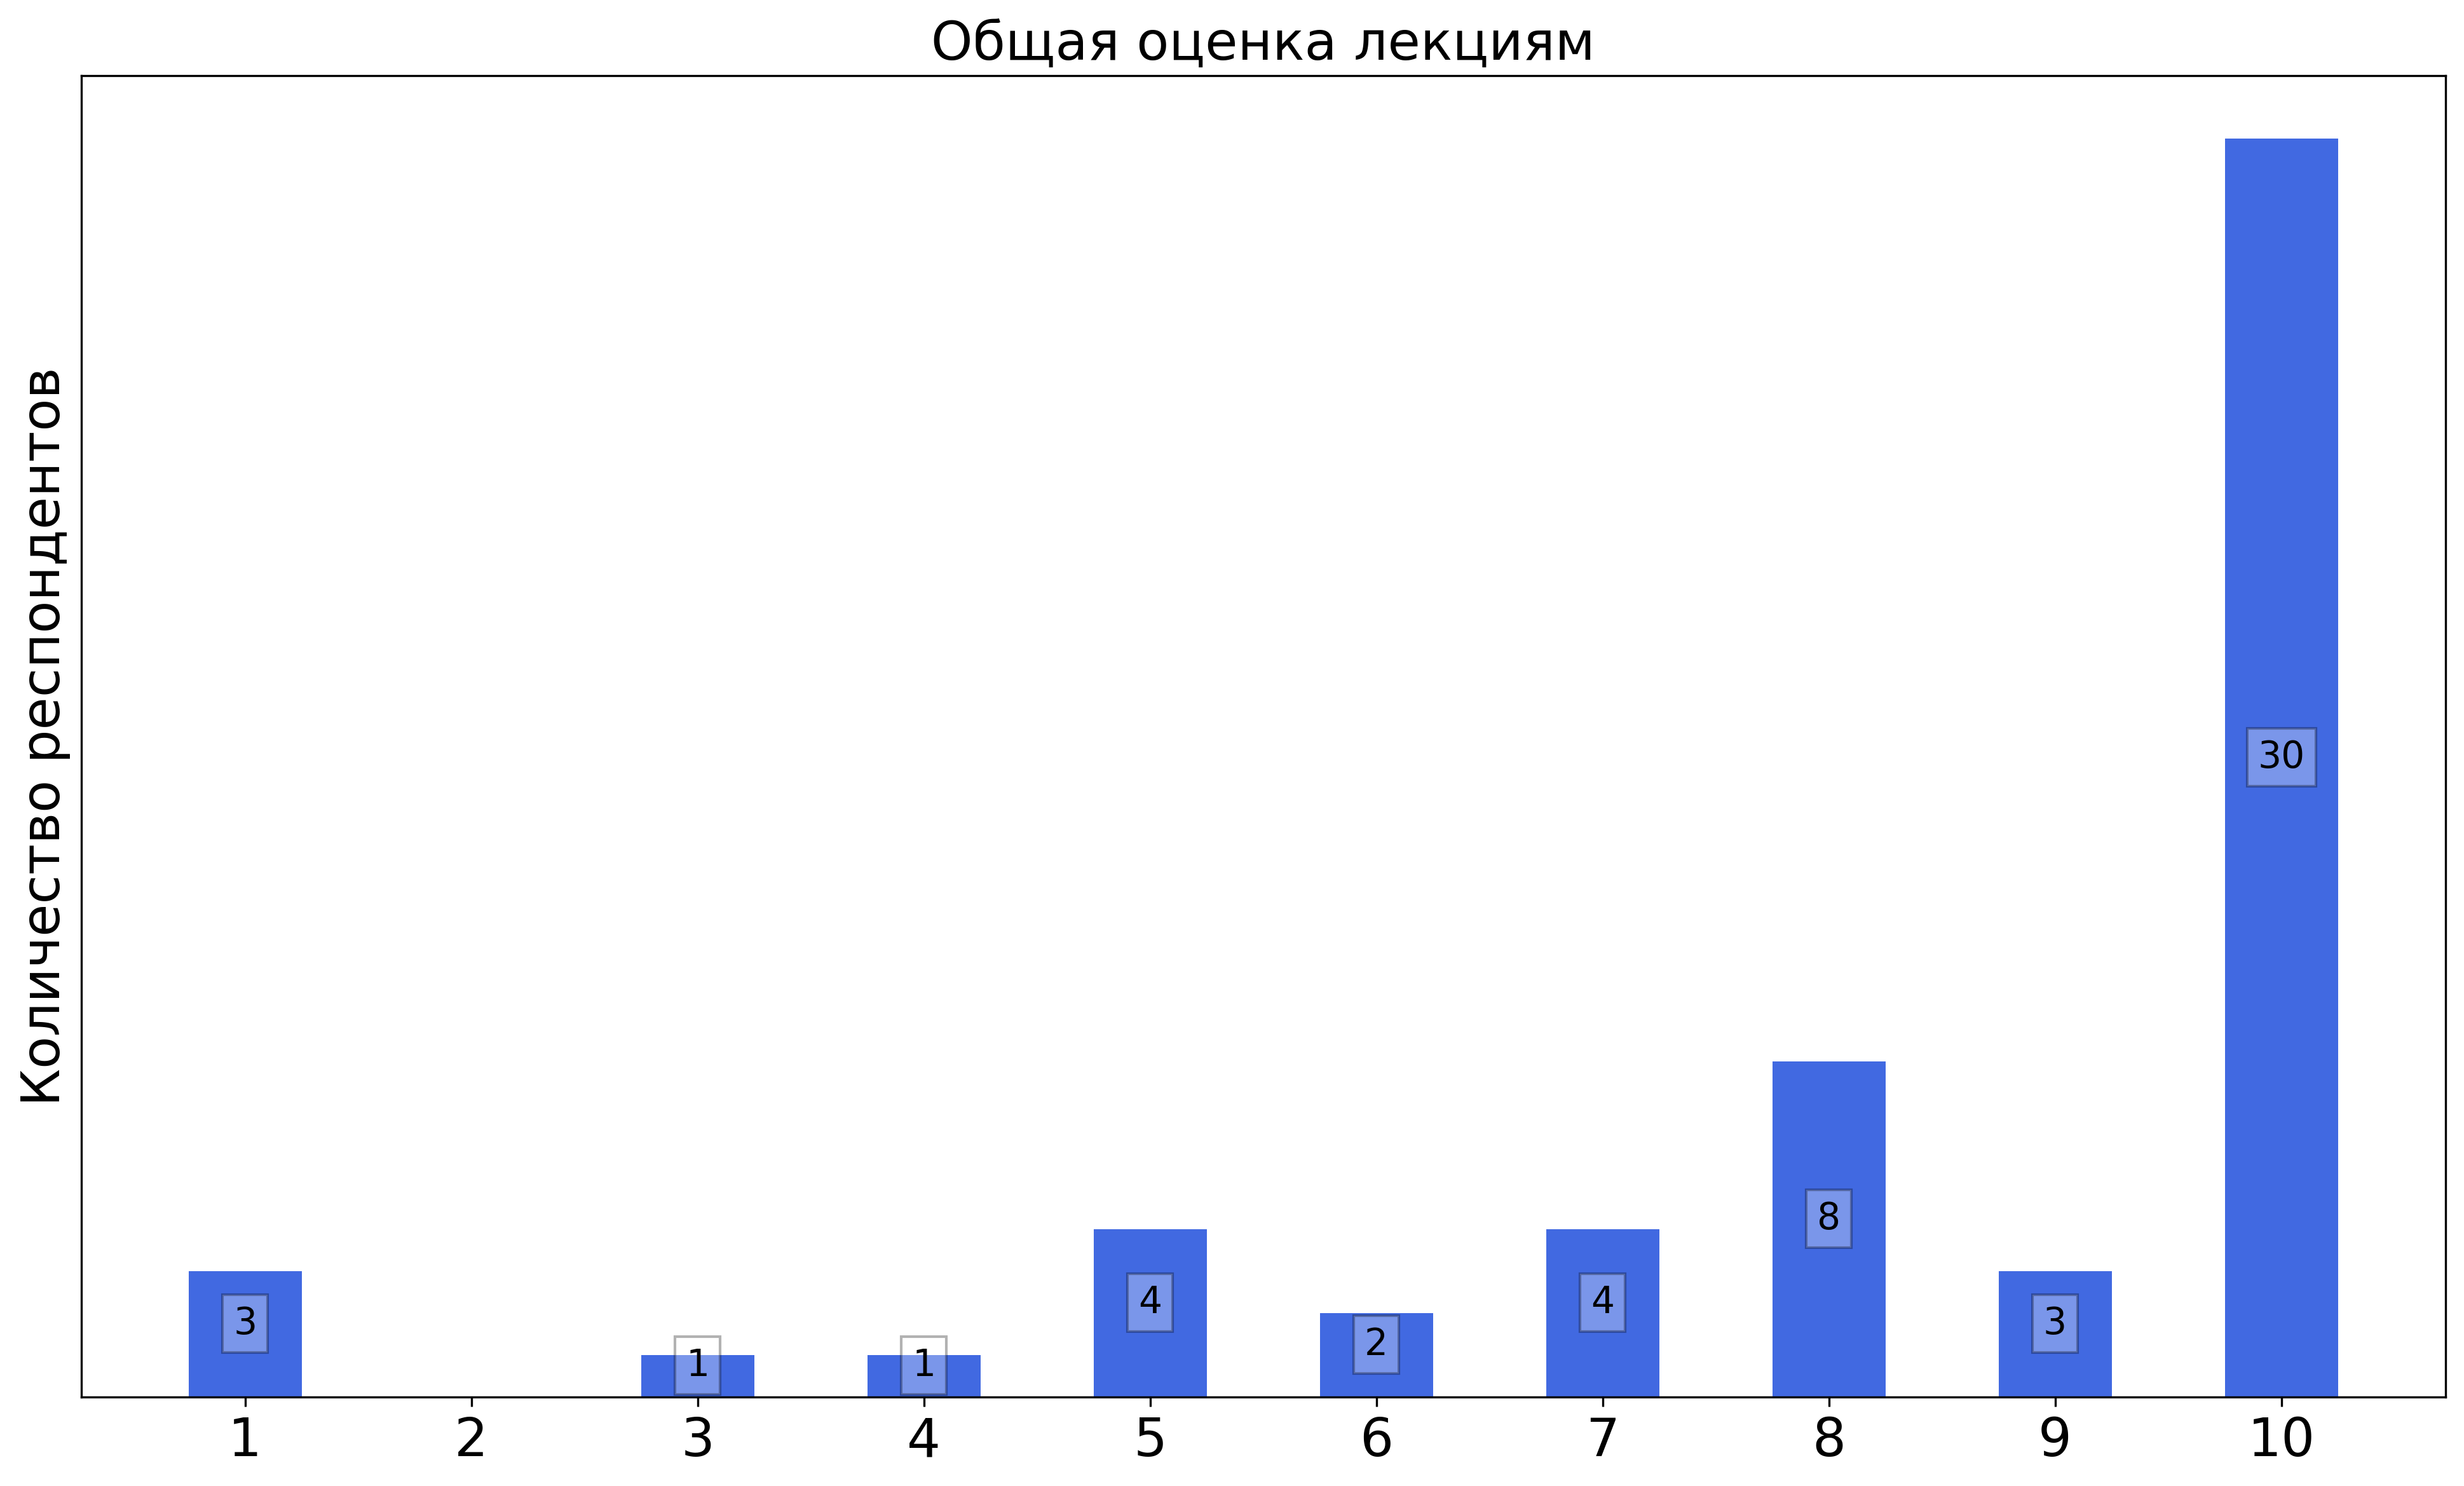
\includegraphics[width=\textwidth]{images/1 course/БЖД/lecturer-marks-3.png}
			\end{subfigure}
			\caption{Оценки респондентов о качестве преподавания лекций по курсу <<БЖД>>}
		\end{figure}
    

    \subsubsection{Прочие комментарии и предложения по улучшению курса}
        \begin{commentbox}
            ничего улучшать не надо, пусть все так и останется для будущих поколений.
        \end{commentbox}

        \begin{commentbox}
            Тяжело в общем сказать о курсе, т.к. всегда разные темы и лекторы. Понравились только когда психолог была и Цыбиков. Остальные (особенно Киреев) это гг
        \end{commentbox}

        \begin{commentbox}
            В начале была не совсем понятна система оценивания, тк разные лекторы говорили разную информацию. Помог только официальный чат и главный лектор
        \end{commentbox}

        \begin{commentbox}
            лучшая лекция та, на которой ты не был
        \end{commentbox}

        \begin{commentbox}
            убрать или уменьшить до минимума 
        \end{commentbox}

        \begin{commentbox}
            Оставьте всё также, либо уберите. Предмет фор фан
        \end{commentbox}

        \begin{commentbox}
            Критерии выставления оценки были довольно расплывчатыми вплоть до конца семестра. На лекциях порой рассказывали интересные вещи, но серьёзно слушать весь курс не имеет смысла.
        \end{commentbox}

        \begin{commentbox}
            Было интересно послушать разных преподавателей, у всех разные темы и своя методика. Некоторые были душные, а некоторые прям класс. Тесты и посещаемость халява, так что в плюсе и те, кто хотят послушать про разные интересные темы, и те, кто вообще забивают. Формат понравился
        \end{commentbox}
